
\subsection{Single Burst}

In the case of a single impulsive burst of star formation, the mass
and energy injection rate per unit stellar mass at time $t$ after the
burst are given, respectively, by
\begin{align} 
  \dot{\bar{m}}(t) &= f_{\rm TO} \dot{m}_{\rm TO} + f_{\rm OB}
  \dot{m}_{\rm OB}\\
% + f_{\rm MS} \int_{m_0}^{m_{\rm T}(t)}
%$  \dot{m}(\Mstar, t) \mu|_{\Mstar} {\rm d}\Mstar
%}{\bar{m}_*}\label{eq:mdotImp}
\dot{\bar{e}}(t) &=f_{\rm OB} \, \dot{e}_{\rm OB}(t)+ f_{\rm MS}
\int_{m_0}^{m_{\rm T}(t)} \frac{\vw^2(\Mstar, t) \dot{m}(\Mstar, t)
  \mu|_{\Mstar} {\rm d}\Mstar}{\bar{m}_*},
  \label{eq:edotImp}
\end{align} 

In the top line, the first term corresponds to mass injection due
winds from post-main sequence stars. The second term corresponds to
mass injection due to stellar winds from massive and O and B
stars. For the latter we use population synthesis calculations by
\citet{VossDiehl+:2009a}. From the bottom panel of their Figure 7, the
stellar wind mass loss rate per massive star can be approximated to within
a factor of a few by

\begin{equation}
\dot{\mathcal{M}}=
\begin{cases}
10^{-6.5} \Msun {\rm yr^{-1}} & t < 4 Myr\\
10^{-5.4} \Msun {\rm yr^{-1}} \left(\frac{t}{4\times 10^6 {\rm
       yr}}\right)^{-3} & 4 {\, \rm Myr} \leq t \leq 40 {\, \rm Myr}. \\
0 & t>40 {\rm Myr}
\end{cases}
\end{equation}

We neglect the mass injection due to stellar winds for times $t\lsim
4$ Myr. $\dot{m}_{\rm OB}=f_{8} \dot{\mathcal{M}}/\bar{m}_{\star}$,
where $f_{8} =2.6 \times 10^{-3}$ is the fraction of the stellar mass
with $M_{\star} > 8M_{\odot}$ and $m_{\star}=0.35 \Msun$ is the mean
stellar mass for our assumed Salpeter IMF, $\mu\sim M_\star^{-2.35}$.



For the mass loss rate from post-main sequence winds, we take

\begin{equation}
  \dot{m}_{\rm TO}=\frac{\Delta M(t) |\dot{M}_{\rm TO}(t)|
    \mu|_{M_{\rm TO}(t)}}{\bar{m}_{\star}}  \,\,  t \geq {\rm 40 Myr},
\end{equation}

and 0 for earlier times. By truncating $\dot{m}_{\rm TO}$ at 40 Myr, we
are ignoring the non-steady mass injection by type II supernovae.

The quantity of mass lost in PMS winds $\Delta M(t)$ is estimated from
the expression given by \citet{CiottiOstriker:2007a} (their eq.~[10]),
\begin{align}
\Delta M=
\begin{cases}
0.945 M_{\rm TO}-0.503 & M_{\rm TO} < 9 \Msun\\
 M_{\rm TO}-1.4 \Msun &  M_{\rm TO} \ge 9 \Msun,
\end{cases}
\end{align}
where $M_{\rm TO}$ is the turn-off mass, which at time $t < t_{\rm h}$ is calculated as
\begin{align}
\log(M_{\rm TO})/M_{\odot} =0.24 + 0.068 x^2-0.34 x+4.76 e^{-4.58 x},
\end{align}
where $x=\log(t/10^9 {\rm yr})$.  This functional fit is designed
to reproduce the results of \citet{MaederMeynet:1987a} (their Table 9)
for massive stars while asymptoting to the formula provided by
\citet{CiottiOstriker:2007a} (their eq.~[9]) for intermediate and late
times ($t \gsim 10^8$ years).

The first term in equation~\eqref{eq:edotImp} corresponds energy
injection from massive O \& B stars, while the second term accounts
for energy injection from stars on the lower main sequence. Both terms
have a thermalization efficiency, $f$, which w e talk to be $1$. Note
we do not account for energy from Type II supernovae. 

Winds from lower main sequence stars only dominate the energy
injection a late times ~10 Gyr after an impulsive burst of star
formation. Even with 100\% thermalization efficiency these winds could
not thermally stabilize the CNM. Thus, we could not describe this
regime within our steady formalism.

The MS wind mass loss rate $\dot{m}(\Mstar, t)$ is calculated based on
the generalization of Reimer's law
\begin{align}
  \dot{m}=4 \times 10^{-13} \frac{L_* R_*}{\Mstar} \Msun \pyear,\
\end{align}
where  $R_*$, $L_*$, $T_{\rm eff}$ and $g_*$ are the stellar radius,
luminosity, effective temperature, and surface gravity, respectively, the latter normalized to its solar value $g_{\odot}$.  The stellar radius and luminosity are estimated as (\citet{Kippenhahn&Weigert90}; Figs.~22.2) 22.3)
\begin{align}
L_*=
\begin{cases}
L_{\odot} (\Mstar/\Msun)^{3.2} & \Mstar > \Msun \\
L_{\odot} (\Mstar/\Msun)^{2.5} & \Mstar \le \Msun
\end{cases}
\end{align}
\begin{align}
R_*=
\begin{cases}
R_{\odot} (\Mstar/\Msun)^{0.57} & \Mstar > \Msun \\
R_{\odot} (\Mstar/\Msun)^{0.8} & \Mstar \le \Msun
\end{cases}
\end{align}
The wind velocity of main sequence winds is assumed to equal $v_w
(\Mstar, t) =
v_{w,\odot}(M_{\star}/M_{\odot})^{1/2}(R_{\star}/R_{\odot})^{-1/2}$,
i.e.~scaling as the stellar escape velocity and normalized to the
velocity of the solar wind $v_{w,\odot} = 430$ km s$^{-1}$; this
produces an effective wind heating velocity for main sequence winds
alone of $\sim 100$ km s$^{-1}$ for $\tau_{\star} \sim t_{\rm h}$,
close to the value found by \citet{NaimanSoares-Furtado+:2013a} for
globular clusters based on a more sophisticated population synthesis
treatment.

The rate of energy injection due to winds from massive
stars, $\dot{e}_{\rm OB}(t) = f_{8}\dot{\mathcal{E}}/\bar{m}_*$, where
$f_{8} =2.6 \times 10^{-3}$ is the fraction of the stellar mass with
$M_{\star} > 8M_{\odot}$ for our assumed Salpeter IMF.  Here
$\dot{\mathcal{E}} (t)$ is the energy injection rate per massive star,
which we estimate as
\begin{align}
\dot{\mathcal{E}} (t)=  1.3 \times 10^{36} {\rm erg\,s^{-1}}
\begin{cases}
  1 & t<4 \times 10^6 {\rm yr}\\
  \left(\frac{t}{4 \times  10^6\,{\rm yr}}\right)^{-3.73} &  4\times
  10^{6} {\rm yr}  \le t \le 10^{8} {\rm yr},\\
  0 & t > 10^8 {\rm yr}
\end{cases}
\label{eq:voss}
\end{align}
based on the results of \citet{VossDiehl+:2009a} (their Fig.~7, top
panel), who use a population synthesis code to simulate the mass and
energy injection into the ISM from an OB association. {\bf AG--should
  just truncate the energy injection at $10^7$ years. Explain why
  turn-off energy injection is negligible in lower mass stars.}


The effective wind velocity in the limit of an impulsive star
formation may then be written as
\begin{align}
\bar{v}_w(t)=2 \dot{\bar{e}}(t)/\dot{\bar{m}}(t)
\label{eq:vwImp}
\end{align}
while 
\begin{align}
\eta = \dot{\bar{m}}(t) \th
\label{eq:etaImp}
\end{align}
 Figure~\ref{fig:vwImp} shows the values of $\bar{v}_w(t)$ and $\eta(t)$ as a function of stellar age, $\tau_{\star}$.

\begin{figure}
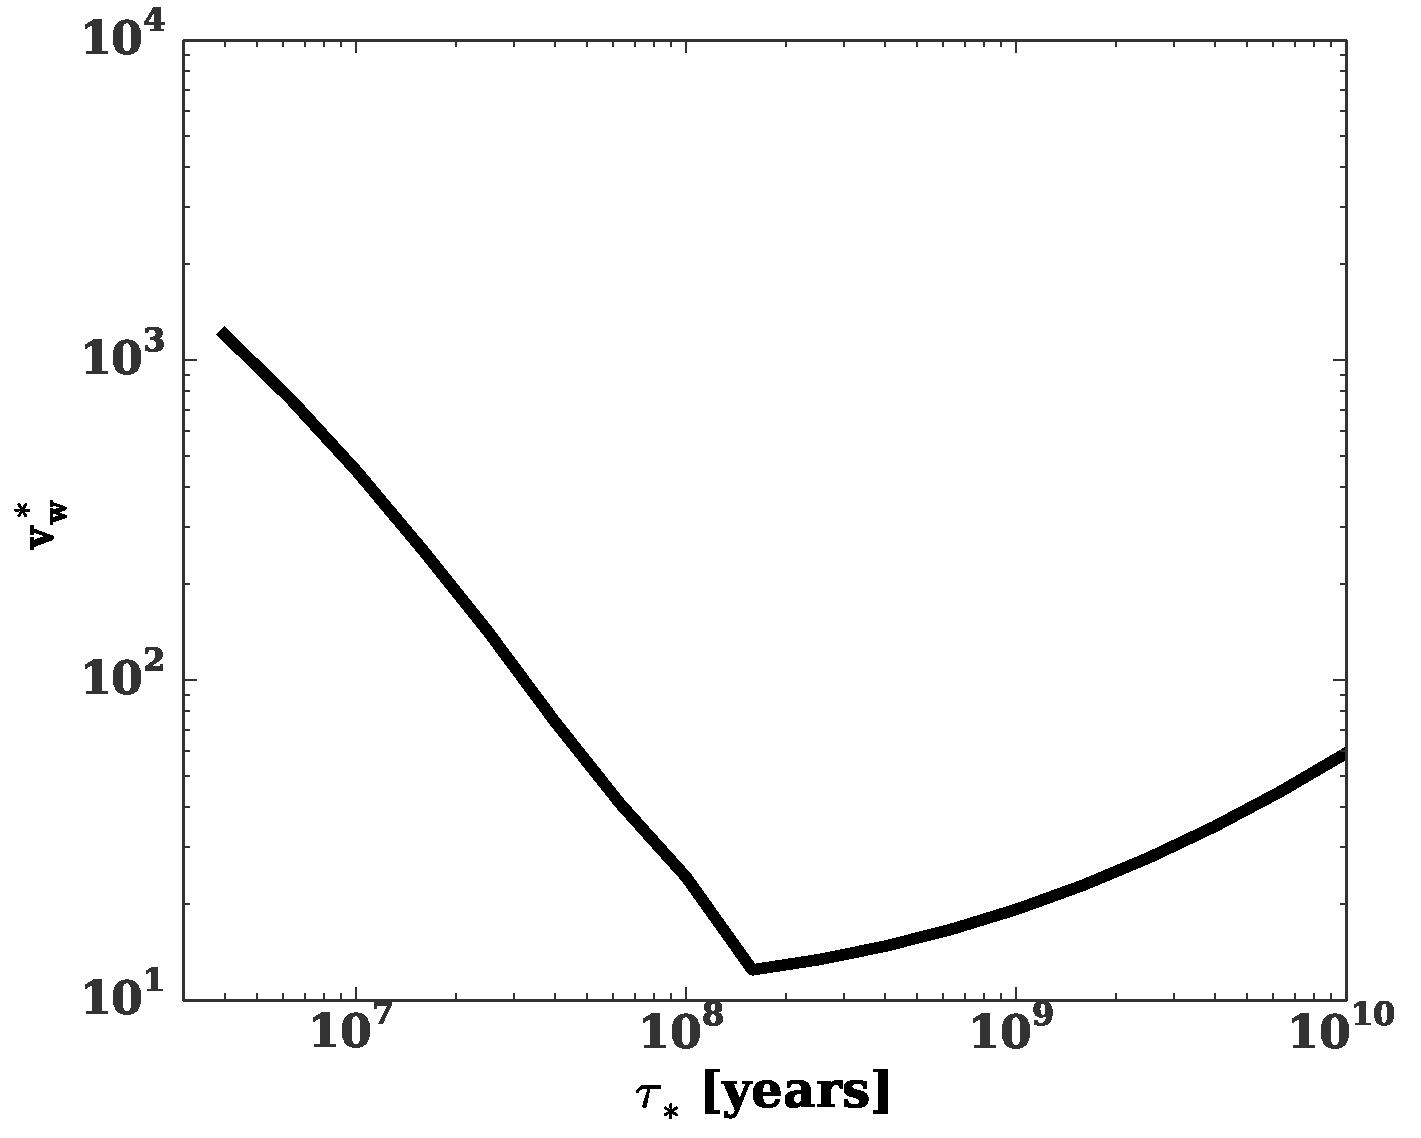
\includegraphics[width=\columnwidth]{vwImp.pdf}
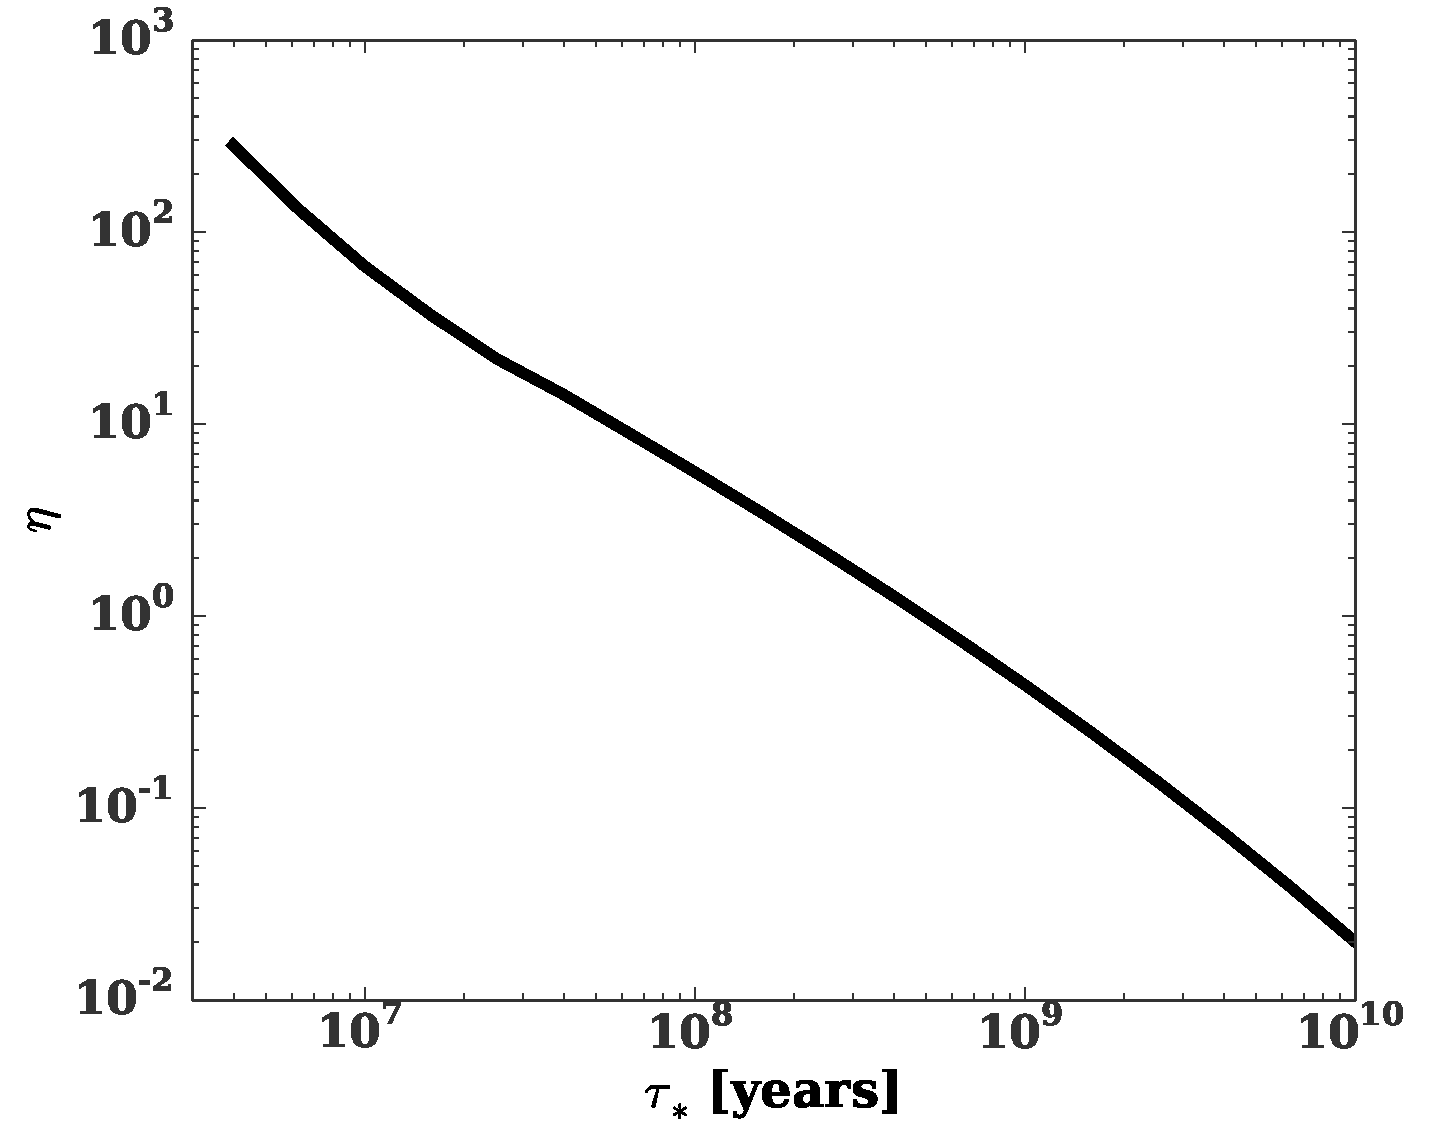
\includegraphics[width=\columnwidth]{etaImp.pdf}
\caption{\label{fig:vwImp} Effective heating rate, $v_w^{\star}$, and mass loss parameter, $\eta$ (eq.~[\ref{eq:q}]), resulting from stellar winds from a stellar population of age $\tau_{\star}$.}
\end{figure}



\subsection{Over Star Formation History}
Generalizing to an arbitrary SFH $S(t)$, the total rate of mass and energy input can be written as
\begin{align} 
  \dot{M}(t) &= \int_0^t S(t_1) \dot{\bar{m}}(t-t_1){\rm
      d}t_1 \label{eq:MDotSFH}\\
  \dot{E}(t) &= \int_0^t S(t_1) \dot{\bar{e}}(t-t_1){\rm
      d}t_1, \label{eq:EDotSFH}
\end{align}
resulting in a wind heating parameter of 
\begin{align}
  v_w^2(t) &=2 \dot{E}(t)/\dot{M}(t).
\end{align}
The mass return parameter will be
\begin{align}
\eta = \frac{\dot{M}(t)}{\int_0^t S(t_1) {\rm d}t_1} \th
\end{align}

 \begin{figure}
  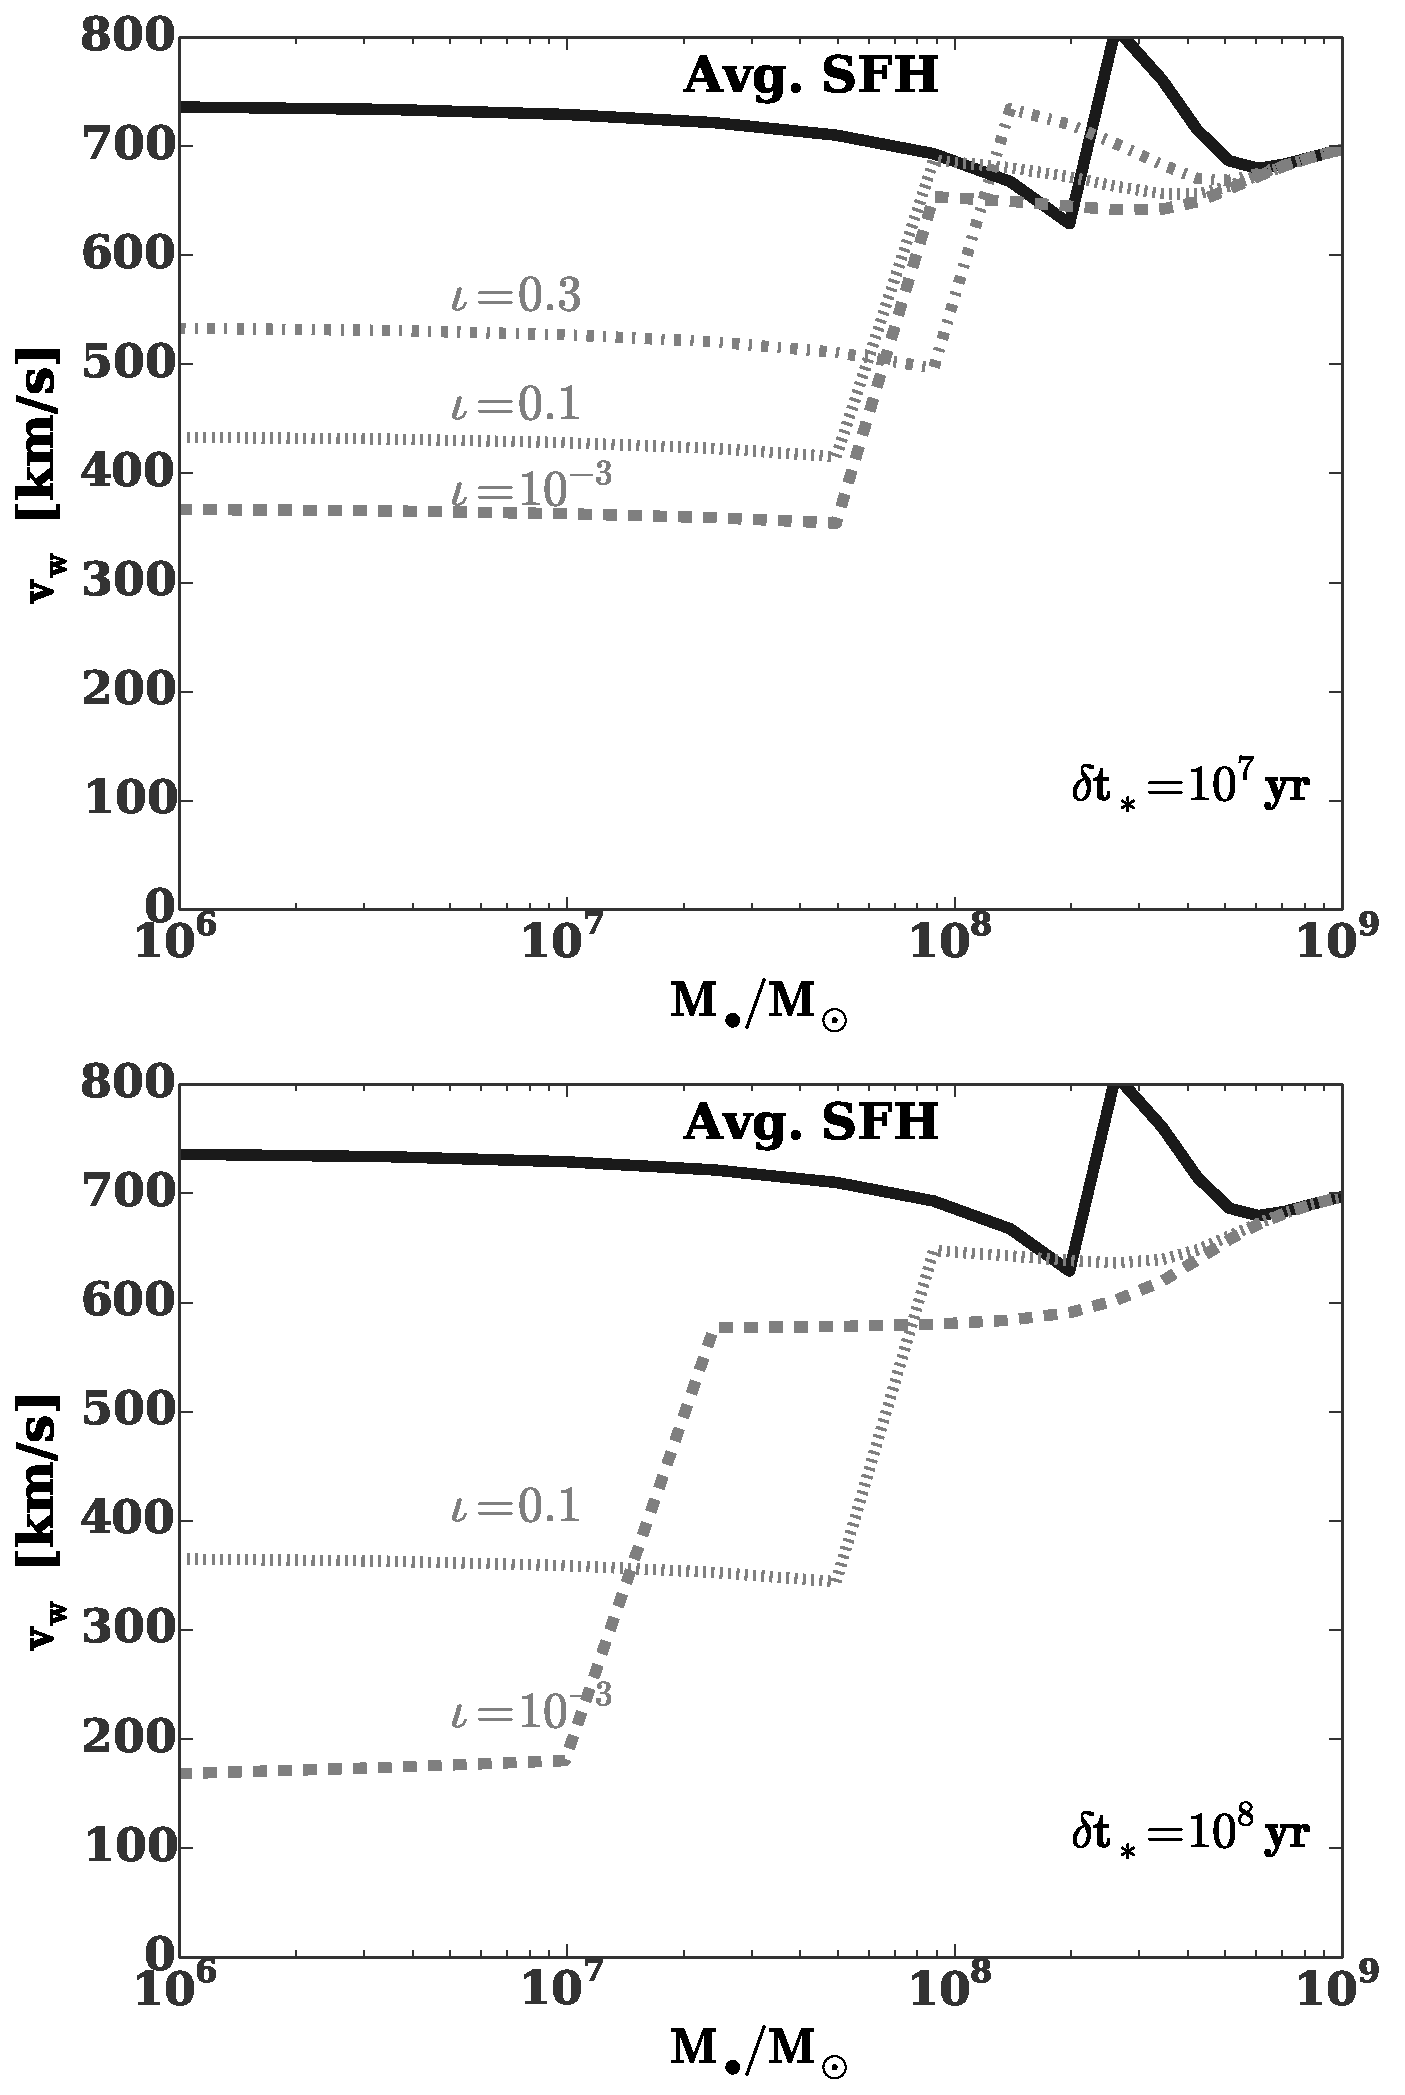
\includegraphics[width=\columnwidth]{bumpy.pdf}
  \caption{\label{fig:NickPlot2} Effective wind velocities for
    nonstandard star formation histories.  The black curves shows, for
    reference, $v_{\rm w}$ calculated using the halo-averaged $S(t)$,
    and gray curves show wind heating resulting from perturbed star
    formation histories given by equation~\eqref{eq:sfrPerturbed}. In
    the top panel the star formation rate declines for a time, $\delta
    t_*=10^{7}$ years to fractions $\iota= 0.001$ (dashed), $\iota
    =0.1$ (dotted), and $\iota = 0.3$ (dot-dashed) of the halo
    averaged value. The bottom panel shows results for $\delta
    t_*=10^{8}$ years and $\iota$=0.001 (dashed) and 0.1 (dotted).}
  \end{figure}
  We estimate the stellar wind heating provided by the {\it average}
  star formation history of galaxies of a given $\Mbh$ using the
  results of \citet[eqs.~17-20]{MosterNaab+:2013a}.  Note that the
  star formation histories in \citet{MosterNaab+:2013a} are in terms
  of halo mass. For a given $\Mbh$ we assign the halo mass whose star
  formation history would produce a bulge consistent with the
  $\Mbh-M_{\rm bulge}$ relationship from \citet{McConnellMa:2013a}.  A
  slight complication occurs for the largest mass halos, where much of
  the $z=0$ stellar mass has been acquired through accretion of
  satellite halos rather than {\it in situ} star formation.  To
  accommodate this, we incorporate analytic fits for mass accretion
  histories, taken from \citet[their eqs.~21-23]{MosterNaab+:2013a},
  assuming that the age distribution of the accreted stars is equal to
  the age distribution of those formed {\it in situ}.  This assumption
  may be conservative if the primary galaxy's accretion history is
  dominated by minor mergers with younger stellar populations.  On the
  other hand, the dynamical friction inspiral time for small satellite
  galaxies is quite long, generally much greater than the $\sim
  10^7~{\rm yr}$ for which young stars can dominate the heating
  budget.  The mass of stars accreted for halo masses, $M_{\rm halo}< 3
  \times 10^{12} \Msun$, and redshifts, $z>4$, is small and is neglected.

  To find the total mass ($\Mdot'(t)$) and energy ($\dot{E}'(t)$)
  injection rates, including the contribution of accreted stars, we
  add a convolution of the specific mass and injection rates with the
  accretion history $A(t)$ to the mass and energy injection rates from
  star formed in-situ.  Thus,

\begin{align}
\Mdot '(t)&=\Mdot(t)+\int_{0}^{t} A(t_{\rm acc}) \frac{\Mdot(t_{\rm acc})}
{\int_{0}^{t_{\rm acc}} S(t_1) dt_1} {\rm dt_{ acc}}\\
\dot{E}'(t)&=\dot{E}(t)+\int_{0}^{t} A(t_{\rm acc}) \frac{\dot{E}(t_{\rm acc})}
{\int_{0}^{t_{\rm acc}} S(t') dt_1} {\rm dt_{acc}}.
\end{align}

The corresponding wind heating parameter $v_w'$ and mass return
parameter, $\eta'$, will be given by

\begin{align}
\eta'&=\frac{\Mdot'(t)}{\int_0^t S(t_1) {\rm d}t_1+\int_0^t A(t_1) {\rm
    d}t_1} \th\\
v_w'^2&=2 \frac{\dot{E}'(t)}{\Mdot'(t)}.
\end{align}

Figure \ref{fig:NickPlot2} shows how the wind heating varies as star formation histories deviate from their halo-averaged values.  In particular, we show
\begin{align} 
  \dot{\mathcal{M}}(t) &= \int_0^t \mathcal{S}(t_1) \dot{\bar{m}}(t-t_1){\rm
      d}t_1\\
  \dot{\mathcal{E}}(t) &= \int_0^t \mathcal{S}(t_1) \dot{\bar{e}}(t-t_1){\rm
      d}t_1,\\
  \mathcal{V}_w^2(t) &=2 \dot{\mathcal{E}}(t)/\dot{\mathcal{M}}(t).
\end{align}
In these equations, 
\begin{equation}
\mathcal{S}(t) = S(t) \times
\left(\frac{2}{\pi}(1-\iota)\arctan(t/\delta t_{\star}) + \iota
\right).
\label{eq:sfrPerturbed}
\end{equation}
This function convolves the recent ($z \approx 0$) halo-averaged star
formation history with local variation to give a more pessimistic
estimate for the value of $\tilde{v}_{\rm w}$.  In particular,
replacing $S(t)$ with $\mathcal{S}(t)$ reduces the recent star
formation rate to a fraction $\epsilon$ of its halo-averaged value,
and does so for a characteristic time $\delta t_{\star}$ into the
past.  As we can see in Fig. \ref{fig:NickPlot2}, this dramatically
lowers the effective wind speed when both $\delta t_{\star} \gtrsim
10^7 ~{\rm yr}$ and $\epsilon \lesssim 0.1$, but otherwise has too
modest of an effect to change the thermal stability properties of the
flow (although the location of $r_{\rm s}$ and the value of $\dot{M}$
may change significantly).


%%% Local Variables: 
%%% mode: latex
%%% TeX-master: "ms"
%%% End: 
